\documentclass{standalone}
\usepackage{tikz}

\begin{document}

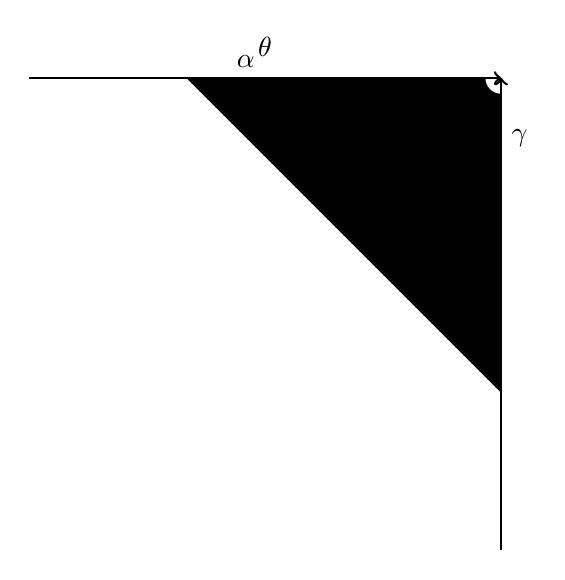
\begin{tikzpicture}[scale=2]
    % Set the origin and coordinates for the triangle
    \coordinate (O) at (-1, 1);
    \coordinate (A) at (-3, 1);
    \coordinate (B) at (-1, -1);

    % Draw the black triangle
    \fill[black] (A) -- (O) -- (B) -- cycle;

    % Draw the black dot at the right angle
    \fill[white] (O) circle (0.1);

    % Define points for the angles
    \coordinate (C) at (-4, 1);
    \coordinate (D) at (-2, 1);
    \coordinate (E) at (-1, 0);
    \coordinate (F) at (-1, -2);

    % Draw the smaller angles
    \draw[thick, ->] (C) -- (O) node[midway, above left] {$\alpha$};
    \draw[thick, ->] (D) -- (O) node[midway, below right] {$\beta$};

    % Draw the larger angle
    \draw[thick, ->] (E) -- (O) node[midway, above right] {$\gamma$};
    \draw[thick, ->] (F) -- (O) node[midway, below left] {};

    % Label the angles
    \node at (-2.5, 1.2) {$\theta$};

\end{tikzpicture}

\end{document}